% !TEX encoding = UTF-8
% !TEX TS-program = pdflatex
% !TEX root = ../tesi.tex

%**************************************************************
\chapter{Strumenti utilizzati}
\label{cap:strumenti-utilizzati}
%**************************************************************

\section{Strumenti di sviluppo}
\subsection{Visual Studio Code}
\begin{figure}[ht]
    \centering
    
\includegraphics[height=2cm]{vsc_logo}
    \caption{Logo di Visual Studio Code}
\end{figure} \aCapo{}
\vsc{} è un editor per codice sorgente, sviluppato da \textit{Microsoft} servendosi del framework \textit{Electron}, disponibile per Windows, Linux e macOS. Le sue funzionalità comprendo supporto per debugging, syntax highlighting, intelligent code completion, snippets, code refactoring, e integrazione con Git. \\
Gli utenti possono configurare tema, macro, preferenze e installare estensioni che ne aumentano le funzionalità aggiungendo ad esempio il supporto ai maggiori linguaggi di porgrammazione attualmente presenti.\\
Nella \textit{Stack Overflow 2021 Developer Survey}, \vsc{} è risultato essere l'IDE più popolare, adottato dal 70\% degli intervistati. {\tiny Fonte: \href{https://en.wikipedia.org/wiki/Visual_Studio_Code}{Wikipedia}}\\
\E{} inoltre presente e molto comoda l'estensione di \flutter{} che, tra le altre cose, permette di gestire direttamente in gui i vari dispositivi (smartphone, browser o emulatore) sui quali installare e lanciare l'app che si sta programmando.

\subsection{Android Studio}
\begin{figure}[ht]
    \centering
    
\includegraphics[height=2cm]{as_logo}
    \caption{Logo di Android Studio}
\end{figure}\aCapo{}
\textit{Android Studio} è l'IDE ufficiale del sistema operativo di Gooogle, sostituendo Eclipse dal 2015, costruito sul software IntelliJ di JetBrains e progettato specificatamente per lo sviluppo Android. \E{} disponibile per Windows, Linux e macOS.\\
Il 7 maggio 2019 Kotlin rimpiazzò Java come linguaggio consigliato per Android, favorendo un'integrazione ancora maggiore con JetBrains che, appunto, ha sviluppato e prodotto Kotlin stesso. {\tiny Fonte: \href{https://en.wikipedia.org/wiki/Android_Studio}{Wikipedia}}\\
Personalmente ho cercato nonostante tutto di programmare il più possibile su \vsc{} preferendolo quindi ad \textit{Android Studio} in virtù della sua maggiore leggerezza e delle sue più ampie possibilità di personalizzazione.

\subsection{Dart}
\begin{figure}[ht]
    \centering
    
\includegraphics[height=2cm]{dart_logo}
    \caption{Logo di Dart}
\end{figure} \aCapo{}
Dart è un linguaggio di programmazione sviluppato da Google per il client development, ovvero per web e mobile app, e può anche essere impiegato per la costruzione di applicazione desktop e server.\\
\E{} un linguaggio object-oriented, class-based, garbage-collected, strongly-typed e con una sintassi nello stile di C. Può compilare sia codice macchina che JavaScript e supporta interefacce, mixins, classi astratte, refined generics e type inference.{\tiny Fonte: \href{https://en.wikipedia.org/wiki/Dart_(programming_language)}{Wikipedia}}\\
Personalmente l'ho trovato elegante e conciso nella sua struttura, e presenta dei vantaggi consistenti come la null protection e le espressioni ternarie.

\subsection{Flutter}
\begin{figure}[ht]
    \centering
    
\includegraphics[height=2cm]{flutter_logo}
    \caption{Logo di Flutter}
\end{figure} \aCapo{}
Flutter è un framework open-source creato da Goole per lo sviluppo della UI di applicazioni cross-platform per Android, iOS, Linux, macOS, Windows, Google Fuchsia e il web partendo da un singolo codebase.\\
Rialsciato a maggio 2017, le applicazioni in Flutter sono scritte in Dart e sfruttano molte delle features avanzate del linguaggio, e le componenti principali del framework sono:
\begin{itemize}
    \item \textbf{Dart platform:} Flutter gira all'interno della Dart Virtual Machine, che si serve di un execution engine just-in-time;
    \item \textbf{Flutter engine:} scritto primariamente in C++, fornisce supporto a basso livello per il rendering e implementa accessibilità, file e network I/O, supporto nativo per i plugin e molto altro;
    \item \textbf{Foundation library:} scritta in Dart, fornisce classi e funzioni di base che vengono usate per costruire gli applcativi in Flutter, come ad esempio le API per la comunicazione con l'engine;
    \item \textbf{Design-specific widgets:} Flutter contiene due famiglie di widget che si conformano a delle specifiche scuole di design: \textit{Material} per Google e \textit{Cupertino} per Apple;
    \item \textbf{Flutter DevTools:} famiglia di tools generici che vengono sfruttati per lo sviluppo di software in Flutter.
\end{itemize}
~\\
Inoltre, una libreria fondamentale per semplificare l'utilizzo di Flutter è \textit{Flutter Hooks}: lo scopo è implementare delle strutture simili agli Hooks di React, consentono di sostituire gli Stateful Widget riducendo il boilerplate code e semplificando la gestione di side-effect e ciclo di vita dei widget grazie alla funzione \textit{useEffect}.

\subsection{Java}
\begin{figure}[ht]
    \centering
    
\includegraphics[height=4cm]{java_logo.png}
    \caption{Logo di Flutter}
\end{figure} \aCapo{}

\subsection{Kotlin}
\begin{figure}[ht]
    \centering
    
\includegraphics[height=1.5cm]{kotlin_logo.png}
    \caption{Logo di Flutter}
\end{figure} \aCapo{}

\subsection{Azure Spatial Anchors}
\begin{figure}[ht]
    \centering
    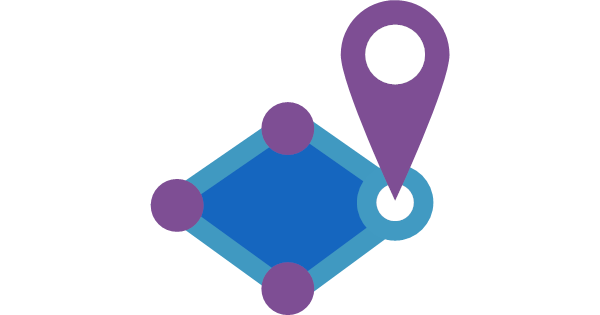
\includegraphics[height=2.5cm]{asa_logo.png}
    \caption{Logo di Flutter}
\end{figure} \aCapo{}

\subsection{ARCore}
\begin{figure}[ht]
    \centering
    
\includegraphics[height=2cm]{arcore_logo.png}
    \caption{Logo di Flutter}
\end{figure} \aCapo{}
%**************************************************************
\section{Strumenti organizzativi}

\subsection{Slack}
\begin{figure}[ht]
    \centering
    
\includegraphics[height=1.5cm]{slack_logo}
    \caption{Logo di Slack}
\end{figure}

Slack è un software che rientra nella categoria degli strumenti di collaborazione aziendale utilizzato per inviare messaggi in modo istantaneo ai diversi membri del team.\\
Slack è utilizzabile da browser, applicazione desktop e applicazione o mobile.\\
Oltre ai messaggi diretti tra i membri è anche possibile creare diversi canali in modo da separare le conversazioni per argomento, per esempio nel nostro caso utilizzavamo due canali: \#frontend, \#backend.\\
Slack inoltre permette di integrare nel sistema di messaggistica anche altri servizi, come per esempio Github o Jira.

\subsection{Jira}
\begin{figure}[ht]
    \centering
    
\includegraphics[height=3cm]{jira_logo.png}
    \caption{Logo di Jira}
\end{figure}

Jira è un software utilizzato per gestire il lavoro collaborativo, segue il principio agile e permette di creare ticket e gestire degli sprint settimanali.\\ Nel nostro caso chiunque poteva aprire un ticket nella sezione \textit{TODO} e assegnarlo a chi di dovere, specificandone i dettagli. Quando il ticket veniva preso in carico lo si spostava nell' apposita sezione \textit{IN PROGRESS} e una volta terminato veniva chiuso nella sezione \textit{DONE}. In questo modo ognuno sa in quale stato è il prodotto e a cosa sta lavorando ogni membro del team.


\subsection{Github}
\begin{figure}[ht]
    \centering
    
\includegraphics[height=3cm]{github_logo}
    \caption{Logo di GitHub}
\end{figure}

GitHub è un servizio di hosting per progetti software ed è una implementazione del sistema di versionamento distribuito Git.\\ Il sito è principalmente utilizzato dagli sviluppatori, che caricano il codice sorgente dei loro programmi e lo possono rendere disponibile al resto degli utenti. Questi ultimi possono interagire con lo sviluppatore tramite un sistema di \textit{issue tracking}, \textit{pull request} e commenti che permette di migliorare il codice del \textit{repository} risolvendo bug o aggiungendo funzionalità.
